\chapter{Technische Umsetzung}
\section{Aufbau des Backends}
\section{Beschreibung der verwendeten Services}


\section{Beschreibung der verwendeten APIs}
\subsection{BoardGameGeek XML API }

Die BoardGameGeek XML API bietet eine Schnittstelle zum Zugriff auf eine Vielzahl von Informationen rund um Brettspiele,
die auf BoardGameGeek.com, einer umfangreichen Datenbank und Community für Brettspiel-Enthusiasten,
verfügbar sind. Diese API ermöglicht es Entwicklern druch verschiedene Endpoints auf Spielinformationen,
Benutzerkollektionen und Forendiskussionen zuzugreifen. Dabei zu beachten ist, dass die API die Antwort als XML-Format weitergibt. 
Da häufig mit JSON gearbeitet wird ist eine mögliche Umformung der Daten sinnvoll.

\large Suchfunktion

Eine der drei benutzten Endpunkte ist die `/xmlapi/search`-Funktion bei der Nutzer als Input einem spezifischen Suchterm eingeben.
Als Ergebnis enthält man eine Liste an Brettspielen in XML Format, deren Namen oder Alias im Suchbegriff enthalten war.
Die Suchfunktion Antwort enthält folgende Informationen:
\begin{itemize}
    \item {objectId des Brettspiels}
    \item {Name des Brettspiels}
    \item {Erscheinungsjahr des Brettspiels}
\end{itemize}

Die reale Ausgabe für den fiktiven Suchterm ``Frika'' würde somit folgendes zurückgeben: 
\begin{figure}[h]
    \centering
    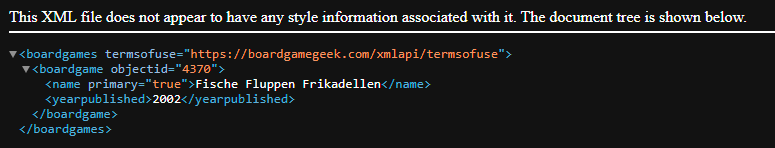
\includegraphics[width=1\textwidth]{graphics/Search_API.png}
    \caption{Ergebnis der `/xmlapi/search`-Funktion bei Suchterm Frika}
    \label{fig:Search_API}
\end{figure}

 \large Detaillierte Spielinformationen

Der zweite Endpunkt ist die `/xmlapi/boardgame/<gameid>`-Funktion und dient dazu,
detaillierte Informationen zu einem Brettspiel zu erhalten. Nutzer könnten hier noch einige weitere Parameter mitgeben um spezifische Informationen zu erhalten, jedoch ist dies in unserem Projekt nicht notwendig, da die Ergebnisse schon detailliert genug sind.
Die gameId ist hierbei der Input, ist gleichzusetzen mit der objectId und kann aus des oben erhaltenen Ergebnisses der Suchfunktion entnommen werden.
Die detaillierten Spielinformationen enthalten folgende Informationen:
% Reduzieren des Abstands zwischen den Punkten
\begingroup
\setlength{\itemsep}{-1pt} % Setzt den Abstand zwischen den Punkten auf 0pt
\setlength{\parskip}{-1pt} % Optional: Reduziert den Abstand zwischen Absätzen
\begin{itemize}
    \item objectId: String
    \item yearPublished: String
    \item minPlayers: String
    \item maxPlayers: String
    \item playingTime: String
    \item minPlayTime: String
    \item maxPlayTime: String
    \item age: String
    \item description: String
    \item name: Array (String)
    \item publisher: Array (String)
    \item averageWeight: String
    \item averageRating: String
    \item thumbnail: String (URL to thumbnail image)
    \item usersRated: String
\end{itemize}
\endgroup

Es ist zu erkennen, dass der Name und der Publisher Arrays sind. Dies lässt sich darauf zurückführen, dass es mehrere Namen für dasselbe Spiel gibt (teilweise auch in anderen Sprachen) und mehrere Entwicklet beteiligt sein können.

\large Game of the Day

Der dritte Endpunkt im Bunde ist die `xmlapi2/hotoverall`-Funktion. Sie gibt die top 50 Spiele mit besonders guter Bewertung und Beliebtheit zurück.
Dabei werden genau fünf unterschiedliche Informationen aufgeführt:
\setlength{\itemsep}{-1pt}
\setlength{\parskip}{-1pt}
\begin{itemize}
    \item id: String (objectId von vorher earlier)
    \item rank: String (Ranking Position der Top 50 Spiele)
    \item thumbnail: String (URL to thumbnail image)
    \item name:  String        
    \item yearpublished 
\end{itemize}

Im Anschluss kann ebenfalls mit der ObjectId eine Anfrage für detaillierte Informationen gestartet werden, die dann auf der Infopage angezeigt werden. 

\subsection{MongoDB API}

In diesem Teil wird nur der externe Aufruf auf den selbsterstellten MongoDB API-Endpunkt behandelt. 
Der Interne Aufbau der MongoDB wird in der Beschreibung der App aufgeführt. Es gibt insgesamt drei Zugriffsmethoden für jede Collection auf die MongoDB: 
searchGamesWishlist(), searchGamesInventory(), addToWishlist(gameData), addToInventory(gameData), removeFromWishlist(objectId), removeFromInventory(objectId)\bigskip


Die Get Methode bezieht sich af den HTTP Endpoint ``http://localhost:8999/wishlisht'' oder beziehungsweise ``\ldots/inventory'' und liefert eine Liste aus JSON-Elementen zurück.
Für das hinzufügen von Brettspielen wird die HTTPClient Methode POST benutzt und die gameData übergeben, wobei Gamedata ein Objekt des Modells Boardgame.ts ist. 

\begin{center}
    \begin{lstlisting}[caption={Löschaufruf der MongoDB API}, label=lst:jscode]
    this.http.delete(`${this.inventoryUrl}/${objectId}`)
\end{lstlisting}
\end{center}


\subsection{Verwendung der APIs im Projekt selbst}

Die Definition der Methoden zum aufrufen der API-Endpunkte ist in dem   File ``board-game.service.ts'' des ``services''-Ordner zu finden.
Dazu wird das HTTPClient Modul importiert und es wird ein htttp.get Aufruf mit den jeweiligen Parametern durchgeführt. Da das Ergebnis in Form einer XML-Datei vorliegt und es vorteilhafter ist mit einem JSON-Format zu arbeiten wird zu Beginn eine Transfarmation des Formats in die JSON Form durchgeführt.
Dies geschieht konkret durch das importierte Modul ``xml2json''. \bigskip 

Die daraufhin vorliegende JSON kann nun dem Modell game.ts, boardgame.ts oder randomtopgame.ts zugewiesen werden. Also eine initialisierung einer Liste von Objekte dieser Modelle basierend auf dem spezifischen API-Aufruf.
Im folgenden wird dann Array als return Element der Funktion definiert. Dies ermöglicht es erstmalig ein subscribe auf die Funktion zu legen und auf der benötigten Page anzuzeigen. \bigskip 

Die konkrete Verwendung der APIs auf den folgenden Pages ist wiefolgt:

\begin{itemize}
    \setlength{\itemsep}{-1pt}
    \setlength{\parskip}{-1pt}
    \item Homepage
        \begin{itemize}
        \item Game of the Day mit `xmlapi2/hotoverall`-Funktion
        \end{itemize}
    \item Searchpage
        \begin{itemize}
        \item Suchfunktion mit `/xmlapi/search`-Funktion
        \end{itemize}
    \item Inventory, Wishlist
        \begin{itemize}
        \item MongoDB mit `http://localhost:8999/inventory`-Funktion oder `.../wishlist` 
        \end{itemize}
    \item Infopage
    \begin{itemize}
    \item Detaillierte Spielinformationen mit `/xmlapi/boardgame/<gameid>`-Funktion 
    \end{itemize}

\end{itemize}

\section{Anleitung zum Starten der Applikation}
